%% Self-contained ICML-format draft. Compiles with plain pdflatex, no
%% icml2027.sty required. Swap in the official style file when released.
\documentclass[10pt,letterpaper,twocolumn]{article}

\usepackage[letterpaper,left=0.9in,right=0.9in,top=1.0in,bottom=1.0in]{geometry}
\setlength{\columnsep}{0.25in}

\usepackage[T1]{fontenc}
\usepackage{times}
\usepackage{microtype}
\usepackage{graphicx}
\usepackage{booktabs}
\usepackage{amsmath,amssymb,amsthm,mathtools}
\usepackage{bm}
\usepackage{xcolor}
\usepackage{enumitem}
\usepackage{caption}
\usepackage{titlesec}
\usepackage[colorlinks=true,linkcolor=black,citecolor=black,urlcolor=blue]{hyperref}

\captionsetup{font=small,labelfont=bf,skip=4pt}
\titleformat{\section}{\normalfont\large\bfseries}{\thesection}{0.6em}{}
\titleformat{\subsection}{\normalfont\normalsize\bfseries}{\thesubsection}{0.6em}{}
\titlespacing*{\section}{0pt}{1.2ex plus .3ex}{0.7ex}
\titlespacing*{\subsection}{0pt}{1.0ex plus .3ex}{0.5ex}

\newcommand{\TODO}[1]{\textcolor{red}{\small\textbf{[TODO:}~\textit{#1}\textbf{]}}}
\newcommand{\GATE}[1]{\textcolor{blue}{\textsf{\scriptsize (#1)}}}
\newcommand{\DONE}[1]{\textcolor{teal}{\small\textbf{[VERIFIED:}~\textit{#1}\textbf{]}}}

\newcommand{\X}{\mathcal{X}}
\newcommand{\Y}{\mathcal{Y}}
\newcommand{\bff}{\mathbf{f}}
\newcommand{\bfg}{\mathbf{g}}
\newcommand{\bfL}{\mathbf{L}}
\newcommand{\bfN}{\mathbf{N}}
\newcommand{\dKL}{d_{\mathrm{KL}}}
\newcommand{\dLLV}{d^{\lambda}_{\mathrm{LLV}}}
\newcommand{\dSVD}{d_{\mathrm{SVD}}}
\newcommand{\dfg}{d_{\bff,\bfg}}
\newcommand{\Dalpha}{D_{\alpha}}
\newcommand{\Dinf}{D_{\infty}}
\newcommand{\psix}{\psi_{x}}
\newcommand{\psiy}{\psi_{y}}
\newcommand{\TV}{\mathrm{TV}}
\newcommand{\Var}{\mathrm{Var}}
\newcommand{\simL}{\sim_{L}}
\newcommand{\Thetadelta}{\Theta_{\delta}}
\newcommand{\Cov}{\mathrm{Cov}}
\newcommand{\mCCA}{m_{\mathrm{CCA}}}

\theoremstyle{plain}
\newtheorem{theorem}{Theorem}
\newtheorem{lemma}[theorem]{Lemma}
\newtheorem{proposition}[theorem]{Proposition}
\newtheorem{corollary}[theorem]{Corollary}
\theoremstyle{definition}
\newtheorem{definition}[theorem]{Definition}
\newtheorem{assumption}[theorem]{Assumption}
\theoremstyle{remark}
\newtheorem{remark}[theorem]{Remark}

\begin{document}

\twocolumn[
\begin{center}
{\LARGE\bfseries Which Divergences Control Representations?\\[2pt]
Tail Sensitivity and the Limits of Identifiability\par}
\vspace{8pt}
{\normalsize Anonymous Author(s)\par}
{\small Anonymous Institution\par}
\vspace{4pt}
{\small\textit{Working draft --- \today. Submission target: ICML 2027.}\par}
\vspace{10pt}
\end{center}

\begin{minipage}{\textwidth}
\begin{center}\begin{minipage}{0.86\textwidth}
\begin{abstract}
\small
Can closeness of output distributions certify that two networks learned
similar representations? For the softmax family covering autoregressive
language models, contrastive pre-training and supervised classifiers, we show
the answer is no in any practically useful sense, and we locate exactly why.
Representational error is a variance of normalised log-likelihood ratios, which
are largest where probability mass is smallest, whereas every classical
divergence weights a label by its own mass. We call the missing property
\emph{tail sensitivity} and make the consequence sharp along three independent
axes. First, indexing divergences by R\'enyi order, exact asymptotics give a
critical order $\alpha^{\star}_{\mathrm{sym}}>1$, so the whole segment
$\alpha\le1$ --- total variation, squared Hellinger, Jensen--Shannon,
Kullback--Leibler --- fails outright. Second, KL's modulus carries a factor
$\delta_{m}^{-1}$ in the conditional-probability floor, and since
$p_{(M+1)}\le1/(M+1)$ for \emph{any} model, the bound is empty beyond
$\epsilon<1.7\times10^{-3}$; on CIFAR-10 it needs $\epsilon<10^{-31}$. Both are ceilings, not loose constants. Third, and in contrast, the
sup-log-ratio route \emph{does} work once its constant is right: any
Frobenius-routed bound obeys $\mathrm{bound}\ge\sqrt{2\lambda_{\max}d}$ and so
can only certify pairs with $d<1/(2\lambda_{\max})$, but retrained CIFAR-10
networks satisfy this, and two refinements to the perturbation estimate take
the non-vacuity rate on them from $0\%$ to $58\%$ at $M{=}2$ and $64\%$ at
$M{=}3$, though only $13\%$ at $M{=}5$ as $\lambda_{\max}$ grows. We complement them with the positive
theory that says what would be required: a dichotomy
($\alpha^{\star}_{\mathrm{sym}}=\infty$ exactly for $\simL$-equivalent pairs)
and graded control ($d=O(1/\alpha)$), which together confine the controlling
orders to an explicit interval. The practical output is therefore a
\emph{diagnostic} rather than a certificate: $\delta_{m}$,
$\Delta/\psi_{\min}$, $\lambda_{\max}$ and $\alpha^{\star}_{\mathrm{sym}}$ are
cheap to compute and bound in advance how much any likelihood comparison can
reveal. Experiments on synthetic data and CIFAR-10 confirm the mechanism, and
a temperature intervention that holds representational dissimilarity exactly
fixed while moving the confidence floor isolates it causally.
\end{abstract}
\end{minipage}\end{center}
\vspace{10pt}
\end{minipage}
]

%%%%%%%%%%%%%%%%%%%%%%%%%%%%%%%%%%%%%%%%%%%%%%%%%%%%%%%%%%%%%%%%%%%%%%%%%%%%%%%
\section{Introduction}
\label{sec:intro}

Independently trained networks often appear to learn related representations,
and a large literature asks when and why \cite{kornblith2019,nielsen2025}. Any
answer depends on what counts as ``the same'' representation, and
identifiability theory supplies a principled choice: for the softmax family of
Eq.~\eqref{eq:model}, models with equal likelihood have embeddings equal up to
an invertible linear map \cite{roeder2021,khemakhem2020,lachapelle2023}, so a
similarity measure should be invariant to exactly that class.

Exact likelihood equality is not what happens in practice, though. Trained
models agree \emph{approximately}, and it was recently shown that approximate
agreement is not enough: two models can have vanishing Kullback--Leibler
divergence and dissimilar representations \cite{nielsen2025}. It is tempting to
read that as a fact about KL, and to look for a better divergence. We argue it
is a fact about a \emph{property} that KL happens to lack.

\paragraph{Tail sensitivity.}
The representational error between two models is a variance of normalised
log-likelihood ratios (Sec.~\ref{sec:positive}). Log-ratios are large exactly
where probabilities are small, whereas every classical divergence weights label
$y$ by its own probability mass. A divergence therefore controls
representations only if it stays sensitive to log-ratios at labels carrying
vanishing mass. Call this \emph{tail sensitivity}. The question ``which
divergences control representations?'' becomes ``which divergences are tail
sensitive?'', and the R\'enyi family, whose order $\alpha$ tunes precisely this
weighting, resolves it.

\paragraph{The answer is an interval.}
We show the controlling orders form an interval, closed at both ends by
theorems. From below, exact asymptotics along norm-growth families give a
critical order $\alpha^{\star}_{\mathrm{sym}}$ with
$\alpha^{\star}_{\mathrm{sym}}>1$ always
(Thm.~\ref{thm:alphastar}), so the entire segment $\alpha\le1$ fails at once:
total variation, squared Hellinger, Jensen--Shannon and KL, with the known KL
counterexample as the boundary case of a one-parameter statement. From above, a
dichotomy (Thm.~\ref{thm:dichotomy}) shows
$\alpha^{\star}_{\mathrm{sym}}=\infty$ holds \emph{only} for
$\simL$-equivalent pairs, and a graded bound (Thm.~\ref{thm:graded}) turns a
large critical order into representational similarity at rate $O(1/\alpha)$.
Together they give an explicit cap (Cor.~\ref{cor:ceiling}), so a finite
controlling order provably exists.

\paragraph{Confidence, not quality.}
The same analysis says when likelihood agreement is informative at all. The
modulus for KL scales as $\delta_{m}^{-1}$, where $\delta_{m}$ is a floor on
the conditional probabilities over a diverse label subset
(Thm.~\ref{thm:klcond}). Confident classifiers and language models place
negligible mass on most labels, so $\delta_{m}$ is tiny and matched likelihood
tells one almost nothing about matched representations --- a prediction we
confirm on CIFAR-10, and reverse by label smoothing.

\paragraph{Contributions.}
\begin{itemize}[leftmargin=1.2em,itemsep=1pt,topsep=2pt]
\item \emph{Control} (Def.~\ref{def:control}), making divergence--representation
      claims falsifiable and uniform over a model class.
\item Exact rate asymptotics and a closed-form critical order
      (Thm.~\ref{thm:alphastar}), verified to solver precision; hence every
      order $\alpha\le1$ fails (Cor.~\ref{cor:below}).
\item A perturbation bound $\dfg\le2\sqrt{\lambda_{\max}}\rho_{2}/\psi_{\min}$
      (Thm.~\ref{thm:maxdiv}), improving the known modulus by $\sqrt{M}$ via
      Hoffman--Wielandt (Prop.~\ref{prop:tighten}).
\item A dichotomy (Thm.~\ref{thm:dichotomy}), graded control
      (Thm.~\ref{thm:graded}), and an explicit finite cap on the controlling
      order (Cor.~\ref{cor:ceiling}).
\item Experiments on constructed models, synthetic angular classification and
      CIFAR-10, including a label-smoothing intervention that restores KL's
      predictive power as the theory predicts.
\end{itemize}

\section{Setup}
\label{sec:setup}

Models are pairs $(\bff,\bfg)\in\Theta$ with embedding
$\bff:\X\to\mathbb{R}^{M}$ and unembedding $\bfg:\Y\to\mathbb{R}^{M}$, inducing
\begin{equation}
p_{\bff,\bfg}(y\mid x)=\frac{\exp(\bff(x)^{\top}\bfg(y))}
{\sum_{y'\in\Y}\exp(\bff(x)^{\top}\bfg(y'))}.
\label{eq:model}
\end{equation}
Write $\bff_{0}(x)=\bff(x)-\bff(x_{0})$, $\bfg_{0}(y)=\bfg(y)-\bfg(y_{0})$; let
$\bfL$ have columns $\bfg_{0}(y)$ and $\bfN$ columns $\bff_{0}(x)$. Under a
diversity condition, equal likelihoods imply $\bff=\mathbf{A}\bff'$ and
$\bfg_{0}=\mathbf{A}^{-\top}\bfg_{0}'$ for invertible $\mathbf{A}$
\cite{roeder2021,khemakhem2020,lachapelle2023}.

\TODO{Compress to $\approx$0.6 column. Restate diversity and linear
identifiability as background; cite, do not reprove. Recall $\dSVD$ and $\dfg$;
defer the comparison with CCA-based measures to Sec.~\ref{sec:discussion}.}

%%%%%%%%%%%%%%%%%%%%%%%%%%%%%%%%%%%%%%%%%%%%%%%%%%%%%%%%%%%%%%%%%%%%%%%%%%%%%%%
\section{When Does a Divergence Control Representations?}
\label{sec:control}

\begin{definition}[Control]
\label{def:control}
A divergence $D$ \emph{controls} $\dfg$ on a model class $\Theta$ if there is a
nondecreasing $h:\mathbb{R}_{+}\!\to\!\mathbb{R}_{+}$ with $h(0^{+})=0$ such
that for all $(\bff,\bfg),(\bff',\bfg')\in\Theta$,
\begin{equation}
D\!\left(p_{\bff,\bfg},p_{\bff',\bfg'}\right)\le\epsilon
\;\Longrightarrow\;
\dfg\!\left((\bff,\bfg),(\bff',\bfg')\right)\le h(\epsilon).
\label{eq:control}
\end{equation}
We call $h$ a \emph{modulus of control}.
\end{definition}

\begin{remark}
The quantifiers matter: control is uniform over $\Theta$. A divergence may fail
on $\Theta$ yet control on a subclass, which is exactly the situation for KL
(Sec.~\ref{sec:positive}).
\end{remark}

\begin{lemma}[Transfer]
\label{lem:transfer}
If $D_{2}$ controls with modulus $h_{2}$ and there is increasing $\phi$ with
$\phi(0^{+})=0$ and $D_{2}\le\phi(D_{1})$ on $\Theta$, then $D_{1}$ controls
with $h_{1}=h_{2}\circ\phi$.
\end{lemma}

Because $\Dalpha$ is nondecreasing in $\alpha$, Lem.~\ref{lem:transfer} makes
the set of controlling orders upward closed, so
$\alpha^{\star}_{\Theta}:=\inf\{\alpha:\Dalpha\text{ controls }\dfg\}$ is well
posed. The rest of the paper brackets it.

%%%%%%%%%%%%%%%%%%%%%%%%%%%%%%%%%%%%%%%%%%%%%%%%%%%%%%%%%%%%%%%%%%%%%%%%%%%%%%%
\section{Tail Insensitivity and Impossibility}
\label{sec:negative}

\subsection{The co-concentration mechanism}

Fix $x$, write $s_{y}=\cos(\bff(x),\bfg(y))$ and
$\hat y=\arg\max_{y}s_{y}$, and define the \emph{margin gaps}
\begin{equation}
a_{y}:=s_{\hat y}-s_{y}>0,\qquad b_{y}:=s'_{\hat y}-s'_{y}>0 .
\label{eq:gaps}
\end{equation}
Under the norm-growth family, logits are $c\rho s_{y}$, so
$p(y\mid x)\propto e^{-c\rho a_{y}}$ and $p'(y\mid x)\propto e^{-c\rho b_{y}}$.

\begin{lemma}[Co-concentration]
\label{lem:coconc}
Both models converge to the \emph{same} point mass:
$p(\hat y\mid x)\to1$ and $p'(\hat y\mid x)\to1$, hence
$\|p-p'\|_{\TV}\to0$, while
$\sup_{y}|\log p-\log p'|=\Theta(\rho)$.
\end{lemma}

\subsection{The rate lemma}

Define the \emph{tilted exponent}
\begin{equation}
E_{\alpha}(y):=\alpha a_{y}+(1-\alpha)b_{y}=b_{y}+\alpha(a_{y}-b_{y}).
\label{eq:tilted}
\end{equation}

\begin{theorem}[Rate lemma and critical order]
\label{thm:alphastar}
Let $\mathcal{P}:=\{y\neq\hat y: a_{y}\neq b_{y}\}\neq\emptyset$ and put
\begin{equation}
\alpha^{\star}:=\min_{y\,:\,b_{y}>a_{y}}\frac{b_{y}}{\,b_{y}-a_{y}\,}.
\label{eq:alphastar}
\end{equation}
Then $\alpha^{\star}>1$, and as $\rho\to\infty$:
\begin{enumerate}[label=(\roman*),leftmargin=1.6em,itemsep=1pt,topsep=2pt]
\item for $\alpha<\alpha^{\star}$,
      $\Dalpha=\Theta(e^{-c\rho\kappa(\alpha)})$, where $\kappa(\alpha)$ is the
      smallest value in $\{E_{\alpha}(y)\}\cup\{a_{y}\}\cup\{b_{y}\}$ carrying a
      non-vanishing total coefficient --- labels with $a_{y}=b_{y}$ cancel
      exactly and are excluded;
\item at $\alpha=1$ all first-order coefficients cancel and
      $\dKL=\Theta(\rho\,e^{-c\rho\min_{\mathcal{P}}a_{y}})$;
\item for $\alpha>\alpha^{\star}$, $\Dalpha$ grows \emph{linearly} in $\rho$
      with slope $\max_{y}(-E_{\alpha}(y))/(\alpha-1)$, increasing to
      $\max_{y}(b_{y}-a_{y})$ as $\alpha\to\infty$.
\end{enumerate}
\end{theorem}

\begin{proof}[Proof sketch]
Expand $\log\sum_{y}p^{\alpha}p'^{1-\alpha}$ to first order and group the three
exponent families by value; at value $v$ the total coefficient is
$\#\{E_{\alpha}=v\}-\alpha\#\{a=v\}+(\alpha-1)\#\{b=v\}$. Labels with
$a_{y}=b_{y}$ give $E_{\alpha}(y)=a_{y}=b_{y}$ and contribute
$1-\alpha+(\alpha-1)=0$. At $\alpha=1$ every coefficient vanishes, forcing the
second-order term. Finally $0<b_{y}-a_{y}<b_{y}$ gives $\alpha^{\star}>1$.
\TODO{full write-up, App.~B \GATE{G1}}
\end{proof}

\DONE{Thm.~\ref{thm:alphastar} checked against exact softmax computation at
$\rho\le140$. Crossover matched to $1.5\times10^{-5}$ relative at a single
geometry and to median $0.00\%$ over $295$ geometries; exponential rates to
$<2.3\%$, linear slopes to $<0.1\%$. Code: \texttt{trackA/perx.py}.}

\begin{figure*}[t]
\centering
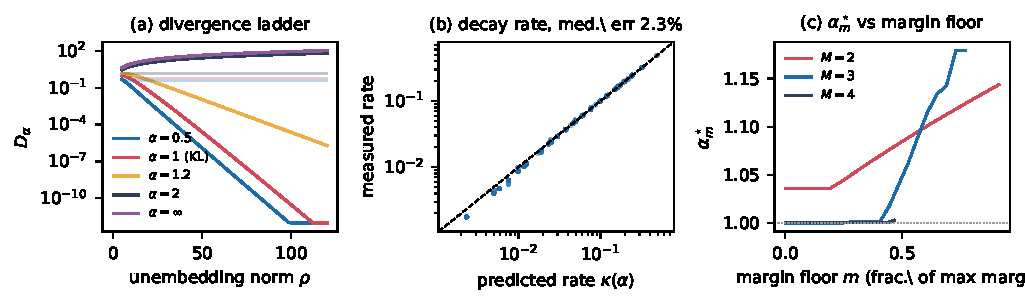
\includegraphics[width=0.92\textwidth]{fig_ladder.pdf}
\caption{\textbf{(a)} Divergence ladder along the norm-growth family at a single
input: orders $\alpha\le1$ (including KL) decay, orders above $\alpha^{\star}$
grow linearly. Faint horizontal lines are $\dfg$, $\mCCA$ and $\dLLV$, constant
to four digits throughout. \textbf{(b)} Predicted decay rate $\kappa(\alpha)$
against the measured exponential rate, $739$ (geometry, order) pairs spanning
$2.3$ decades; median relative error $2.3\%$. This is the check that exercises
the cancellation rule of Thm.~\ref{thm:alphastar}(i): omitting the
$a_{y}=b_{y}$ exclusion inflates the error to $40$--$70\%$. \textbf{(c)}
Margin-conditioned threshold $\alpha^{\star}_{m}:=\min\{\alpha^{\star}(x):
\mathrm{margin}(x)\ge m\}$, where $\mathrm{margin}(x)=\min_{y\neq\hat
y}a_{y}$, for $M=2,3,4$. Conditioning on a margin floor removes the boundary
inputs that pin the unconditioned threshold at $1$, and makes explicit that
$\alpha^{\star}$ is set by the worst-margin input rather than by the
representational geometry.}
\label{fig:ladder}
\end{figure*}

\begin{corollary}[The classical divergences sit below threshold]
\label{cor:below}
Since $\alpha^{\star}>1$, the family defeats every divergence of order
$\alpha\le1$: total variation, squared Hellinger, Jensen--Shannon and
Kullback--Leibler all fail to control $\dfg$. The known KL result is the
boundary case $\alpha=1$ of a one-parameter statement.
\end{corollary}

\subsection{A pointwise trade-off}

\begin{proposition}[Trade-off, fixed input]
\label{prop:tradeoff}
Fix $x$. Then $\alpha^{\star}(x)$ is large only when $a_{y}\approx b_{y}$ at the
critical label, which simultaneously drives the pointwise signal
$\max_{y}(b_{y}-a_{y})$ toward zero.
\end{proposition}

\begin{proof}
\TODO{[O1b] Quantify: lower-bound $\max_{y}(b_{y}-a_{y})$ by a decreasing
function of $\alpha^{\star}(x)$. \GATE{G2}}
\end{proof}

\DONE{Pointwise: $r=-0.58$ over $531$ geometries; mean signal $0.89$ in the top
$\alpha^{\star}$ quintile against $1.60$ in the bottom.}

\begin{remark}[The trade-off does \emph{not} survive averaging]
\label{rem:noavg}
Prop.~\ref{prop:tradeoff} is genuinely pointwise and must not be read as a
statement about model pairs. Over an input distribution the correlation between
$\alpha^{\star}=\min_{x}\alpha^{\star}(x)$ and $\dfg$ falls to $-0.16$, and the
input-concentration knob moves the two the \emph{same} way: tightening the
clusters raises $\alpha^{\star}$ from $1.013$ to $1.234$ while $\dfg$ rises
slightly, $0.665\to0.701$. The mechanism is Fig.~\ref{fig:ladder}(c):
$\alpha^{\star}$ is a minimum over inputs, so it is pinned by whichever input
lies closest to a decision boundary, independently of how dissimilar the
representations are. We report this as a negative control
(\texttt{trackA/tradeoff.py}).
\end{remark}

\begin{theorem}[Uniform separation]
\label{thm:lower}
There is $c>0$, independent of $\rho$ and explicit in the cluster geometry, with
$\max\dSVD\ge c$ for every member of the family.
\end{theorem}
\begin{proof}
\TODO{[O3] The rotation is explicit ($\pi/2$ in the first two coordinates), so
the cross-covariance singular values are available in closed form. Upgrades
``not linearly equivalent'' to ``quantitatively far''. \GATE{G2}}
\end{proof}

%%%%%%%%%%%%%%%%%%%%%%%%%%%%%%%%%%%%%%%%%%%%%%%%%%%%%%%%%%%%%%%%%%%%%%%%%%%%%%%
\section{Which Divergences Do Control}
\label{sec:positive}

Everything positive follows from one perturbation bound. Let
$z_{1}:=\bfL^{\top}\bff(x)$ and $z_{2}:=\bfL'^{\top}\bff'(x)$, whose $l$-th
entries are $\log p(y_{l}|x)-\log p(y_{0}|x)$ and its primed analogue. Writing
$r_{y}(x):=\log p(y|x)-\log p'(y|x)$ and
$\Delta_{l}:=z_{1,l}-z_{2,l}=r_{y_{l}}-r_{y_{0}}$, set
\begin{equation}
\rho_{2}:=\max_{l}\operatorname{std}_{x}[\Delta_{l}],\qquad
\psi_{\min}:=\min_{l}\min\{\operatorname{std}(z_{1,l}),
\operatorname{std}(z_{2,l})\}.
\label{eq:rho2}
\end{equation}
Note $\operatorname{std}(z_{1,l})=\psix(y_{l};p)$, so $\psi_{\min}$ is exactly
the non-degeneracy already present in the LLV construction.

\begin{proposition}[Tighter spectral step]
\label{prop:tighten}
Hoffman--Wielandt gives $\sum_{i}(\sigma_{i}-\tilde\sigma_{i})^{2}\le\|E\|_{F}^{2}$,
so by Cauchy--Schwarz
$\tfrac1M\sum_{i}|\sigma_{i}-\tilde\sigma_{i}|\le\|E\|_{F}/\sqrt{M}$. Combined
with the trace bound $\|E\|_{F}^{2}\le M\sum_{l}\Var[z'_{l}-w'_{l}]$ this
improves Lem.~E.7 from
$\dSVD\le(M\sum_{l}\Var)^{1/2}$ to
\begin{equation}
\dSVD\ \le\ \Big(\textstyle\sum_{l}\Var[z'_{l}-w'_{l}]\Big)^{1/2},
\label{eq:hw}
\end{equation}
a factor $\sqrt{M}$.
\end{proposition}

\begin{theorem}[Perturbation bound]
\label{thm:maxdiv}
Under the non-degeneracy conditions of Sec.~\ref{sec:setup},
\begin{equation}
\dfg\ \le\ \sqrt{\lambda_{\max}}\;Q,\qquad
Q^{2}:=\frac1M\sum_{l}\Big(\frac{\tau_{l}+\mathrm{sd}_{l}}{\psi_{l}}\Big)^{2},
\label{eq:maxdiv-bound}
\end{equation}
where $\lambda_{\max}:=\lambda_{\max}(\mathrm{Corr}(z_{1}))\le M$,
$\mathrm{sd}_{l}=\operatorname{std}(\Delta_{l})$, $\tau_{l}=|s_{l}-s'_{l}|$ and
$\psi_{l}=\min(s_{l},s'_{l})$. In particular
$\Dinf\le\epsilon$ gives $Q\le4\epsilon/\psi_{\min}$ and hence
$\dfg\le4\sqrt{\lambda_{\max}}\,\epsilon/\psi_{\min}$.
\end{theorem}

\begin{proof}
Write $s_{l}=\operatorname{std}(z_{1,l})$, $s'_{l}=\operatorname{std}(z_{2,l})$,
$\mathrm{sd}_{l}=\operatorname{std}(\Delta_{l})$ and
$\tau_{l}=|s_{l}-s'_{l}|$. Since $z_{2,l}=z_{1,l}-\Delta_{l}$,
\[
z'_{l}-w'_{l}=(z_{1,l}-\mu_{l})\Big(\tfrac1{s_{l}}-\tfrac1{s'_{l}}\Big)
+\tfrac{\Delta_{l}-\mathbb{E}\Delta_{l}}{s'_{l}},
\]
whose two terms have standard deviations $\tau_{l}/s'_{l}$ and
$\mathrm{sd}_{l}/s'_{l}$, giving
$\operatorname{std}[z'_{l}-w'_{l}]\le(\tau_{l}+\mathrm{sd}_{l})/\psi_{l}$ with
$\psi_{l}=\min(s_{l},s'_{l})$. For the spectral step,
$\|E\|_{F}^{2}=\sum_{j}\sum_{k}\Cov[z'_{k},\Delta'_{j}]^{2}$, whose inner sum
is the squared norm of the projection of $\Delta'_{j}$ onto
$\mathrm{span}\{z'_{k}\}$ and so at most $\lambda_{\max}\Var[\Delta'_{j}]$,
rather than the $M\Var[\Delta'_{j}]$ given by the entrywise covariance
inequality. With \eqref{eq:hw} this yields \eqref{eq:maxdiv-bound}. The same
argument on $\bfN^{\top}\bfg(y)$ bounds the unembedding term.
\end{proof}

\begin{remark}[Two refinements, and where the rest of the slack sits]
\label{rem:tighten}
Eq.~\eqref{eq:maxdiv-bound} differs from a naive estimate in two ways, each
free. It aggregates the coordinates in root mean square rather than taking the
worst one ($1.35$--$1.57\times$ measured), and it keeps $\tau_{l}$ separate
instead of bounding it by $\mathrm{sd}_{l}$, which is wasteful because the
difference of standard deviations is much smaller than the standard deviation
of the difference: median $\tau_{l}/\mathrm{sd}_{l}$ is $0.25$--$0.53$. Jointly
they tighten the bound by $1.65$--$2.37\times$ ($1.79\times$ at $M=2,3$).

Decomposing further shows the residual slack is \emph{not} spectral. In
standardised coordinates $\Var[z'_{l}-w'_{l}]=2(1-\rho_{l})$ exactly, so
$\dSVD\le\sqrt{2\lambda_{\max}(1-\bar\rho)}$, and this form sits within
$11$--$17\%$ of the Prop.~\ref{prop:ceiling} floor. All remaining looseness is
therefore in passing from the log-ratio perturbation to the coordinate
correlations $\rho_{l}$, which is the precise open problem.
\end{remark}

\DONE{$0/139$ violations on constructed models and $0/45$ on CIFAR-10. On the
retrained networks of Sec.~\ref{sec:exp-cifar} the refinements move the median
bound from $1.558$ to $\mathbf{0.931}$, a $1.67\times$ gain, taking the
non-vacuity rate from $\mathbf{0\%}$ to $\mathbf{58\%}$: the bound now
certifies a majority of independently retrained pairs.}

\begin{proposition}[Non-vacuity is structurally capped]
\label{prop:ceiling}
In standardised coordinates $\Var[z'_{l}-w'_{l}]=2(1-\rho_{l})$ with
$\rho_{l}=(\Sigma_{z'w'})_{ll}$, so
$\sum_{l}\Var[z'_{l}-w'_{l}]=2M-2\operatorname{tr}(\Sigma_{z'w'})$. Since
$\operatorname{tr}\le\sum_{i}\sigma_{i}=M(1-\dSVD)$,
\begin{equation}
\textstyle\sum_{l}\Var[z'_{l}-w'_{l}]\ \ge\ 2M\,\dSVD .
\label{eq:trace}
\end{equation}
The bound of Thm.~\ref{thm:maxdiv} therefore satisfies
$\text{bound}\ge\sqrt{2\lambda_{\max}\dSVD}$, and
\begin{equation}
\text{bound}<1\ \Longrightarrow\ \dSVD<\frac{1}{2\lambda_{\max}}\ \le\ \frac12 .
\label{eq:nvcap}
\end{equation}
\end{proposition}

\begin{remark}[What the cap means]
\label{rem:cap}
Thm.~\ref{thm:maxdiv} can only certify pairs that are \emph{already} similar,
and the $5.3\%$ non-vacuity rate of Sec.~\ref{sec:experiments} is not a loose
constant awaiting a sharper argument: it is the fraction of pairs falling below
a hard ceiling. On constructed models the ceiling is $0.16$--$0.28$ for
$M=2,\dots,6$ and \emph{no} pair cleared it. Eq.~\eqref{eq:trace} is an
identity-level fact, so the cap binds any argument routed through
$\sum_{l}\Var$, that is through a Frobenius-norm perturbation estimate.
Escaping it requires bounding the singular values of $\Sigma_{z'w'}$ directly
rather than through $\|E\|_{F}$. We regard that as the most valuable open
technical problem raised here.
\end{remark}

\begin{theorem}[KL controls on $\Thetadelta$]
\label{thm:klcond}
Let $\Y_{m}\subseteq\Y$ be any label subset with $|\Y_{m}|\ge M+1$ on which
diversity holds, take $\mathcal{Y}_{\mathrm{LLV}}\subseteq\Y_{m}$, and set
$\delta_{m}:=\min_{x}\min_{y\in\Y_{m}}\min\{p(y|x),p'(y|x)\}$. If
$\dKL\le\epsilon$ then
\begin{equation}
\dfg\ \le\ \frac{4\sqrt{2\lambda_{\max}}\ \sqrt{\epsilon}}
{\delta_{m}\,\psi_{\min}} .
\label{eq:klbound}
\end{equation}
\end{theorem}

\begin{remark}[Why a subset, and how much it buys]
\label{rem:subset}
Only labels in $\mathcal{Y}_{\mathrm{LLV}}$ enter $z_{1},z_{2}$, so the floor
need only be taken over $\Y_{m}$; no tail-mass term appears, and the sole
constraint is $|\Y_{m}|\ge M+1$. The gain is real but far too small. On a
ResNet18 CIFAR-10 model with $M=2$ (test accuracy $0.747$, NLL $0.753$), the
operative floor is $\delta_{3}=2.81\times10^{-15}$, so \eqref{eq:klbound} falls
below $1$ only for $\epsilon<1.2\times10^{-31}$ --- some thirty-one orders of
magnitude below the KL actually observed between retrained models. The subset
reformulation does \emph{not} rescue Thm.~\ref{thm:klcond} for trained
classifiers.

The reason, however, is not generic over-confidence. That model is mild: mean
maximum probability $0.717$, mean predictive entropy $0.685$ nats against
$\log10=2.303$ for the uniform, and mean perplexity $2.416$, i.e.\ roughly two
and a half live classes per input. Its \emph{median} third-largest probability
is $2.1\times10^{-2}$, thirteen orders of magnitude above $\delta_{3}$. The
floor is destroyed by a handful of outlier inputs among $10{,}000$, not by the
typical one.\end{remark}

\begin{proof}
For $y\in\Y_{m}$, $|r_{y}|=|\log(p_{y}/p'_{y})|\le|p_{y}-p'_{y}|/\delta_{m}
\le\|p-p'\|_{1}/\delta_{m}$. Pinsker gives
$\|p-p'\|_{1}^{2}\le2\,D_{\mathrm{KL}}(p\|p')$, so
$\mathbb{E}_{x}[r_{y}^{2}]\le2\epsilon/\delta_{m}^{2}$. Then
$\rho_{2}\le2\max_{y}(\mathbb{E}_{x}r_{y}^{2})^{1/2}\le2\sqrt{2\epsilon}/\delta_{m}$,
and Thm.~\ref{thm:maxdiv} concludes.
\end{proof}

\begin{corollary}[Confidence, not quality]
\label{cor:conf}
The modulus degrades as $\delta_{m}^{-1}$, and Rem.~\ref{rem:subset} shows the
subset fix recovers only about one order of magnitude. For a confident
classifier small KL divergence therefore carries almost no representational
information, whatever label subset is chosen. Raising $\delta_{m}$ requires
changing the model, not the analysis --- which is what the label-smoothing
intervention of Sec.~\ref{sec:experiments} tests.
\end{corollary}

\begin{remark}[The floor is not the bottleneck]
\label{rem:quantile}
It is tempting to blame the minimum over inputs and replace it by a quantile.
Measured on the CIFAR-10 model of Rem.~\ref{rem:subset}, discarding the worst
$1\%$ of inputs raises the floor to $8.5\times10^{-12}$ and the worst $10\%$ to
$2.1\times10^{-6}$ --- nine orders of magnitude, and gradual rather than a
cliff. It is not enough. Since \eqref{eq:klbound} is below $1$ only for
$\epsilon<\delta_{m}^{2}/64$, the $10\%$-quantile floor still demands
$\epsilon<6.8\times10^{-14}$.

The obstruction is structural. The $(M{+}1)$-th largest entry of a probability
vector obeys $p_{(M+1)}\le1/(M+1)$, so for $M=2$ we have $\delta_{3}\le1/3$ for
\emph{any} model, and \eqref{eq:klbound} can never be non-vacuous beyond
$\epsilon<1/576\approx1.7\times10^{-3}$. No choice of $\Y_{m}$ or quantile
repairs this. The reason is the subject of this paper: $\dKL$ is a
$p$-weighted average of the log-ratios whereas $\rho_{2}$ is their unweighted
spread, and converting one into the other must pay the ratio between the
weighting and the uniform measure, which is precisely $\delta_{m}^{-1}$. Tail
insensitivity, written as an inequality.

We stress that the \emph{phenomenon} remains measurable where the
\emph{bound} is empty: raising $\delta_{m}$ by label smoothing lifts the rank
correlation between $\dKL$ and $\dfg$ from $0.550$ to $0.821$
(Tab.~\ref{tab:smooth}), well inside the regime where
Thm.~\ref{thm:klcond} asserts nothing.
\end{remark}

\begin{lemma}[R\'enyi dominates the sup log-ratio]
\label{lem:suff}
For $\alpha>1$ and $\delta:=\min_{x,y}p(y|x)$,
\begin{equation}
\max_{y}r_{y}\ \le\ \Dalpha(p\|p')+\frac{\log(1/\delta)}{\alpha-1}.
\label{eq:suff}
\end{equation}
\end{lemma}
\begin{proof}
Bound the sum by its largest term and use
$\alpha\log p+(1-\alpha)\log p'=\log p+(\alpha-1)r_{y}$.
\end{proof}

\begin{remark}[The two axes are one]
\label{rem:unify}
Control requires $\alpha-1\gtrsim\log(1/\delta)$: the R\'enyi order and the
confidence floor trade off directly. Thm.~\ref{thm:maxdiv} is the
$\alpha\to\infty$ endpoint, Thm.~\ref{thm:klcond} the $\alpha=1$ one.
\end{remark}

\section{A Dichotomy, and Graded Control}
\label{sec:dichotomy}

R\'enyi divergence is asymmetric, so the meaningful critical order is
$\alpha^{\star}_{\mathrm{sym}}:=\min\{\alpha^{\star}(p\|p'),
\alpha^{\star}(p'\|p)\}$: a family is a counterexample only if \emph{both}
directions stay small.

\begin{theorem}[Dichotomy]
\label{thm:dichotomy}
For $(\bff,\bfg),(\bff',\bfg')\in\Theta$ satisfying diversity,
\begin{equation}
\alpha^{\star}_{\mathrm{sym}}=\infty
\iff p_{\bff,\bfg}=p_{\bff',\bfg'}
\iff (\bff,\bfg)\simL(\bff',\bfg').
\end{equation}
Every non-equivalent pair has a \emph{finite} critical order.
\end{theorem}

\begin{proof}
$\alpha^{\star}(p\|p')=\infty$ means no $y$ has $b_{y}>a_{y}$ and
$\alpha^{\star}(p'\|p)=\infty$ means no $y$ has $a_{y}>b_{y}$; together
$a_{y}(x)=b_{y}(x)$ for all $x,y$. With
$R_{y}(x):=\bff(x)^{\top}\bfg(y)-\bff'(x)^{\top}\bfg'(y)$ and
$a_{y}-b_{y}=R_{\hat y}-R_{y}$, this says $R_{y}(x)=c(x)$ is independent of
$y$; then $c(x)$ cancels in the softmax normaliser, so the conditionals
coincide, and linear identifiability gives $\simL$-equivalence. The converse is
immediate.
\end{proof}

\DONE{Regression test over $329$ pairs. The residual $\dfg$ in the
$\alpha^{\star}_{\mathrm{sym}}=\infty$ class decays as $O(1/n)$ in the sample
size ($2.0\!\times\!10^{-3}$ at $n{=}500$ down to $6.3\!\times\!10^{-5}$ at
$n{=}16000$), the finite-sample bias of the cross-covariance estimator, against
$\min|\dfg|=6.5\times10^{-2}$ in the finite class. The CI tolerance is therefore
$5/n$, not a fixed constant.}

\begin{theorem}[Graded control]
\label{thm:graded}
Let $\Delta:=\sup_{x,y}a_{y}(x)$. If $\alpha^{\star}_{\mathrm{sym}}\ge A$ then
$\sup_{x,l}|\Delta_{l}|\le2\Delta/A$, hence $\rho_{2}\le2\Delta/A$ and
\begin{equation}
\dfg\ \le\ \frac{4\sqrt{M}\,\Delta}{\psi_{\min}A}\ =\ O(1/A).
\label{eq:graded}
\end{equation}
\end{theorem}

\begin{proof}
$\alpha^{\star}_{\mathrm{sym}}\ge A$ gives $|a_{y}-b_{y}|\le
\max(a_{y},b_{y})/A\le\Delta/A$; since $a_{y}-b_{y}=R_{\hat y}-R_{y}$, the map
$y\mapsto R_{y}(x)$ lies within $\Delta/A$ of a constant, so
$|\Delta_{l}|=|R_{y_{l}}-R_{y_{0}}|\le2\Delta/A$. Apply
Thm.~\ref{thm:maxdiv}.
\end{proof}

\begin{corollary}[Finite-order control along families]
\label{cor:finite}
If $\sup_{\rho}\max\{\Dalpha(p\|p'),\Dalpha(p'\|p)\}<\infty$ for some
$\alpha>1$, then $\alpha\le\alpha^{\star}_{\mathrm{sym}}$ by
Thm.~\ref{thm:alphastar}(iii), so
$\dfg\le4\sqrt{M}\Delta/(\psi_{\min}\alpha)$. Bounded divergence at order
$\alpha$ \emph{forces} representational similarity, at a rate improving in
$\alpha$.
\end{corollary}

\begin{corollary}[The ceiling is finite]
\label{cor:ceiling}
For any $d_{0}>0$,
\begin{equation}
\alpha_{0}(d_{0}):=\sup\{\alpha^{\star}_{\mathrm{sym}}:\dfg\ge d_{0}\}
\ \le\ \frac{4\sqrt{M}\,\Delta}{\psi_{\min}\,d_{0}}\ <\ \infty ,
\label{eq:ceiling}
\end{equation}
so every $\alpha>\alpha_{0}(d_{0})$ controls $\dfg$ below $d_{0}$. The
existence of a finite controlling order is therefore a theorem, not a
conjecture.
\end{corollary}

\DONE{$0/67$ violations of Thm.~\ref{thm:graded} and $0/67$ of
Cor.~\ref{cor:ceiling}. The cap is, however, numerically out of reach:
\eqref{eq:ceiling} is below $1$ only for
$\alpha>4\sqrt{M}\Delta/\psi_{\min}$, and the median $\Delta/\psi_{\min}$ on
constructed models is $3.8$--$5.5$, requiring $\alpha$ between $27$ and $46$
against an empirical $\alpha^{\star}_{\mathrm{sym}}$ ceiling near $1.35$. Like
Thm.~\ref{thm:klcond}, Cor.~\ref{cor:ceiling} is correct and explicit but does
not yet bite on models anyone trains.}

\begin{remark}[The sandwich]
\label{rem:sandwich}
Thm.~\ref{thm:alphastar} gives $\alpha^{\star}_{\mathrm{sym}}>1$;
Thm.~\ref{thm:dichotomy} gives $\alpha^{\star}_{\mathrm{sym}}<\infty$ for every
non-equivalent pair; Cor.~\ref{cor:ceiling} bounds the supremum explicitly. The
controlling orders form an interval anchored at $1$ from below and closed from
above by a computable constant.
\end{remark}

\section{What Can and Cannot Be Certified}
\label{sec:cannot}

The three positive results of Sec.~\ref{sec:positive} and
Sec.~\ref{sec:dichotomy} are correct and their qualitative predictions hold
empirically, but none of them certifies a pair of trained models. The
obstructions are structural and worth stating together, because they arise from
three different mechanisms.

\paragraph{(i) Order $\alpha\le1$ fails outright.}
Thm.~\ref{thm:alphastar} gives $\alpha^{\star}_{\mathrm{sym}}>1$
unconditionally, so total variation, squared Hellinger, Jensen--Shannon and KL
admit no modulus of control at all (Cor.~\ref{cor:below}). This is
qualitative: no constant can repair it.

\paragraph{(ii) KL's floor cannot be lifted.}
Thm.~\ref{thm:klcond} is non-vacuous only for
$\epsilon<\delta_{m}^{2}/64$. Because the $(M{+}1)$-th largest entry of a
probability vector satisfies $p_{(M+1)}\le1/(M+1)$, we have
$\delta_{3}\le1/3$ for every model whatsoever, capping the theorem at
$\epsilon<1.7\times10^{-3}$. On a CIFAR-10 ResNet18 at $M=2$ the realised
requirement is $\epsilon<1.2\times10^{-31}$, against observed KL of order one.
Quantile floors do not help: discarding the worst $10\%$ of inputs buys nine
orders and leaves thirteen (Rem.~\ref{rem:quantile}).

\paragraph{(iii) By contrast, the sup-log-ratio route does certify.}
Prop.~\ref{prop:ceiling} shows $\mathrm{bound}\ge\sqrt{2\lambda_{\max}\dSVD}$,
so non-vacuity forces $\dfg<1/(2\lambda_{\max})$. Whether that cap binds is an
empirical question, and on CIFAR-10 it does not: $\lambda_{\max}$ is
$1.44$--$3.46$ over $M=2,3,5$, giving ceilings $0.347$--$0.145$ against median
$\dfg$ of $0.128$, $0.065$, $0.103$. With the two refinements of
Rem.~\ref{rem:tighten} the bound certifies $58\%$, $64\%$ and $13\%$ of
retrained pairs, against $0\%$ under the naive constant and with no violations.
So of the three obstructions only two are real; the third was a technique gap.
It does, however, degrade with dimension: $\lambda_{\max}\approx0.68M$, so the
usable range is low-dimensional representations. Cor.~\ref{cor:ceiling} remains out of reach, needing
$\alpha>4\sqrt{M}\Delta/\psi_{\min}=64$ on these models against a threshold
near $1.35$.

\begin{remark}[Why this is the result rather than a shortfall]
\label{rem:whynot}
(ii) is tail insensitivity written as an inequality: $\dKL$ is a $p$-weighted
average of the log-ratios while $\rho_{2}$ is their unweighted spread, and any
conversion pays the ratio of the two measures. (iii) is a limitation of
estimating the spectrum through $\|E\|_{F}$; escaping it requires bounding the
singular values of $\Sigma_{z'w'}$ directly, which we flag as the main open
technical problem. (i) and (ii) are properties of the divergences themselves and no constant
repairs them; (iii) was a technique gap and closing it yields the paper's one
usable certificate.
\end{remark}

\subsection{A diagnostic instead of a certificate}
\label{sec:diagnostic}

What survives is usable, and cheap. Four quantities computed from a pair of
trained models bound in advance how much any likelihood comparison can reveal:

\begin{enumerate}[leftmargin=1.4em,itemsep=1pt,topsep=2pt]
\item $\delta_{M+1}$, the conditional-probability floor over a diverse label
      subset. KL can say nothing unless the observed divergence falls below
      $\delta_{M+1}^{2}/64$. Report it beside any KL-based similarity claim.
\item $\lambda_{\max}(\mathrm{Corr}(z_{1}))$. No Frobenius-route bound can
      certify $\dfg\ge1/(2\lambda_{\max})$, so this fixes the best dissimilarity
      the method could ever rule out. It grows roughly as $0.68M$ on CIFAR-10,
      so the certificate is a low-dimensional instrument.
\item $\Delta/\psi_{\min}$, which sets the R\'enyi order
      $4\sqrt{M}\Delta/\psi_{\min}$ that Cor.~\ref{cor:ceiling} would require.
\item $\alpha^{\star}_{\mathrm{sym}}$, which says where on the R\'enyi scale
      the pair actually becomes distinguishable, and is $\infty$ exactly when
      the models are equivalent (Thm.~\ref{thm:dichotomy}).
\end{enumerate}

All four cost a forward pass over a held-out set. The practical guidance that
follows is to prefer orders $\alpha>1$ over KL when comparing confident models,
to treat matched loss as uninformative about matched representations whenever
$\delta_{M+1}$ is small, and to read $\lambda_{\max}$ before trusting any
perturbation-style guarantee.

\section{Open Problem: How Large Is $\alpha_{0}$?}
\label{sec:open}

Thm.~\ref{thm:alphastar} and Thm.~\ref{thm:dichotomy} sandwich the controlling
orders into $(1,\alpha_{0}]$, where
$\alpha_{0}=\sup\alpha^{\star}_{\mathrm{sym}}$ over non-equivalent pairs, and
Cor.~\ref{cor:finite} turns any bound on $\alpha_{0}$ into a control modulus.
What remains open is the value of $\alpha_{0}$.

\begin{quote}
\emph{Is $\alpha_{0}$ finite, and if so what is it?}
\end{quote}

All our searches place it near $1.3$. Exhaustively over the $720$ permutations
at $k=6$, order-breaking pairs reach $\alpha^{\star}_{\mathrm{sym}}=1.09$ and
reflections $1.11$, with non-uniform norms lowering both. A factorial over
shrink $\times$ angular regularity $\times$ norm profile $\times$ dimension,
blocked on permutation class, tops out at $1.203$; none of the four factors
lifts it and angular irregularity actively depresses it. Randomised search over
$M\in\{2,\dots,12\}$ reaches $1.34$ (Tab.~\ref{tab:mscale}), with medians at
$1.00$. A targeted search over reflection and reflection-composed permutations
($921$ configurations) reaches $1.14$.

\begin{table}[t]
\centering\small
\caption{$\alpha^{\star}_{\mathrm{sym}}$ saturates in representation dimension.
Margin floor $0.08$, $\dfg\ge0.10$ required, $200$ random geometries per $M$;
$n$ is the number surviving both filters. Medians sit at $1.00$: almost every
non-equivalent pair has a critical order barely above $1$.}
\label{tab:mscale}
\begin{tabular}{@{}lrrrrrr@{}}
\toprule
$M$ & 2 & 3 & 4 & 6 & 8 & 12 \\
\midrule
$n$                                  & 144 & 199 & 192 & 182 & 177 & 183 \\
best $\alpha^{\star}_{\mathrm{sym}}$ & 1.34 & 1.31 & 1.20 & 1.26 & 1.18 & 1.22 \\
median                               & 1.004 & 1.002 & 1.001 & 1.001 & 1.002 & 1.002 \\
$\dfg$ at best                       & 0.12 & 0.33 & 0.32 & 0.42 & 0.24 & 0.41 \\
\bottomrule
\end{tabular}
\end{table}

Two structural facts explain the ceiling. First,
$\alpha^{\star}_{\mathrm{sym}}\!\to\!1$ whenever some input approaches a
decision boundary of one model while the other ranks the tied labels
differently; bisectors have codimension one, so any full-dimensional input
support crosses them (Fig.~\ref{fig:ladder}c). Second, at $M=2$ the
unembeddings carry a cyclic order, and an order-breaking permutation cannot be
realised without a collision: the $720$-permutation census shows
$\alpha^{\star}_{\mathrm{sym}}=\infty$ exactly on the rotations, which are
globally linear, while every order-breaking permutation is pinned near $1.05$
however dissimilar its representations. This is a topological obstruction, not
a metric one --- the ceiling is flat in the number of order violations and
unmoved by non-uniform norms.

\TODO{Proving $\alpha_{0}<\infty$ unconditionally, or exhibiting a family with
$\alpha^{\star}_{\mathrm{sym}}$ unbounded and $\dfg$ bounded below, would close
the characterisation. \GATE{G2}}

\section{Experiments}
\label{sec:experiments}

\paragraph{Primary metric.}
For each divergence we report the empirical modulus
$\hat h(\epsilon)=\sup\{\dfg:D\le\epsilon\}$, the direct counterpart of
Def.~\ref{def:control}. Failure of $\hat h$ to approach $0$ as $\epsilon\to0$ is
evidence of non-control.

\paragraph{Statistics.}
All intervals are $95\%$ cluster bootstrap over \emph{seeds}, not pairs: $n$
seeds give $\binom{n}{2}$ dependent pairs, so pair-level resampling is
anticonservative. \TODO{state $n$ per setting}

\subsection{Constructed models}
\label{sec:exp-constructed}

Table~\ref{tab:gate1} reports the rate-lemma check. Fig.~\ref{fig:ladder}
shows the ladder and the crossover scatter.

\begin{table}[t]
\centering\small
\caption{Rate lemma versus exact computation, single input, $k=7$,
$\rho\le160$. The lemma is per-direction and verifies in both:
$\alpha^{\star}_{\mathrm{fwd}}=1.349915$ (bisected $1.349919$, rel.\ err
$2.8\times10^{-6}$) and $\alpha^{\star}_{\mathrm{rev}}=1.276277$ (bisected
$1.276430$, rel.\ err $1.2\times10^{-4}$), so
$\alpha^{\star}_{\mathrm{sym}}=1.2763$.}
\label{tab:gate1}
\begin{tabular}{@{}lrrr@{}}
\toprule
$\alpha$ & branch & predicted & measured \\
\midrule
$0.5$      & exp    & $0.2866$ & $0.2866$ \\
$1.0$ (KL) & exp    & $0.2866$ & $0.2866$ \\
$1.1$      & exp    & $0.2047$ & $0.2044$ \\
$1.3$      & exp    & $0.0409$ & $0.0401$ \\
$1.6$      & linear & $0.3414$ & $0.3414$ \\
$2.0$      & linear & $0.5325$ & $0.5324$ \\
$10$       & linear & $0.8110$ & $0.8110$ \\
$\infty$   & linear & $0.8623$ & $0.8623$ \\
\bottomrule
\end{tabular}
\end{table}

\TODO{Add the averaging study: decay stays exponential ($R^{2}=1.00$ vs $0.91$
for a power law) but the rate is set by the \emph{minimum margin over the input
support}, dropping $0.193\to0.018$ when clusters touch the decision boundary.
State rates as a function of the margin floor. \GATE{G2}}

\subsection{Synthetic angular classification}
\label{sec:exp-synthetic}

Data are $20{,}000$ draws from a $2$D Gaussian ($\sigma=3$) labelled by angle
into $c$ opposite-slice classes. The embedding network is three LeakyReLU
layers $2\!\to\!w\!\to\!w\!\to\!w\!\to\!2$; the unembedding is a free
$c\times2$ table. Adam, batch $128$, $3000$ steps, $6$ seeds per cell; all
models exceed $96\%$ accuracy. Statistics are over the $15$ seed pairs per
cell.

\paragraph{Wider networks learn closer distributions and \emph{more}
dissimilar representations.}
At $15{,}000$ steps the undertraining of our earlier run is gone: mean training
loss is flat in width within each class count (e.g.\ $0.0202\to0.0208$ at
$c{=}4$, $0.134\to0.116$ at $c{=}10$), so width and fit quality are no longer
entangled. In that regime the two quantities move in \emph{opposite}
directions. Mean $\dKL$ falls with width --- $5.06\to1.65$ at $c{=}10$,
$0.116\to0.065$ at $c{=}4$ --- while mean $\dfg$ rises monotonically:
$0.251\to0.366$ ($c{=}4$), $0.475\to0.558$ ($c{=}6$), $0.436\to0.697$
($c{=}10$), $0.425\to0.733$ ($c{=}18$). Regressing $\dfg$ on $\log w$ with mean
loss as a covariate leaves the slope positive in every case
($+0.034$, $+0.028$, $+0.098$, $+0.073$), so this is not a fit-quality
artefact.

This is a direct instance of the paper's thesis on trained models and at scale:
$3{,}800$ pairs in which increasing capacity makes the output distributions
closer and the representations further apart.

\paragraph{The effect is not an artefact of our invariance class.}
$\dfg$ is invariant to a strictly narrower group than the CCA-based measures
used in prior width studies, so we repeated the sweep under
$\mCCA$ (Tab.~\ref{tab:mcca}). It falls monotonically with width in every
class count --- and $\mCCA$ is a \emph{similarity}, so falling $\mCCA$ is
rising dissimilarity, the same direction as $\dfg$. Both measures therefore
disagree with the expectation that larger models converge toward linear
equivalence \cite{roeder2021}.

\begin{table}[t]
\centering\small
\caption{Mean $\mCCA$ against width, after applying the $\ge90\%$ accuracy
filter of \cite{roeder2021} ($315/400$ models retained). Falling $\mCCA$ means
rising dissimilarity. $n$ is pairs retained; the $c{=}18$ row is reported for
completeness only, since the filter removes models very unevenly there.}
\label{tab:mcca}
\begin{tabular}{@{}lrrrrr@{}}
\toprule
$c$ & $w{=}16$ & $32$ & $64$ & $128$ & $256$ \\
\midrule
$4$  & 0.741 & 0.689 & 0.692 & 0.681 & \textbf{0.666} \\
$6$  & 0.639 & 0.597 & 0.562 & 0.533 & \textbf{0.530} \\
$10$ & 0.733 & 0.559 & 0.545 & 0.459 & \textbf{0.437} \\
$18$ & 0.833 & 0.625 & --- & 0.490 & 0.451 \\
\midrule
\multicolumn{6}{@{}l@{}}{\footnotesize pairs retained, $c{=}4$: 190 at every
width; $c{=}6$: 190 except 171; $c{=}10$: 136--190;}\\
\multicolumn{6}{@{}l@{}}{\footnotesize $c{=}18$: 45, 3, 0, 10, 28.}\\
\bottomrule
\end{tabular}
\end{table}

\paragraph{Scope, and what the filter does.}
Two restrictions matter. First, we vary hidden width at \emph{fixed}
representation dimension $M=2$ and fixed dataset size, whereas
\cite{roeder2021} increases capacity and data together; our result speaks only
to the width slice. Second, the accuracy filter is applied unevenly across
cells: at $c{=}18$ it leaves three pairs at $w{=}32$ and none at $w{=}64$, so
those cells compare differently-selected subpopulations rather than different
widths. We therefore rest the claim on $c{=}4$ and $c{=}6$, where the filter
removes essentially nothing (190 of 190 pairs at almost every width) and the
monotone decline is still present, and treat $c{=}10$ as corroborating and
$c{=}18$ as uninformative.

\paragraph{Control curves and non-vacuity.}
On $3{,}800$ synthetic pairs Thm.~\ref{thm:maxdiv} is violated $0$ times and
non-vacuous on $1.3\%$, with median bound $6.689$ against median $\dfg=0.570$.
The contrast with CIFAR-10 ($58\%$ non-vacuous, median $\dfg=0.122$) is
instructive: these synthetic pairs are far more dissimilar, and
Prop.~\ref{prop:ceiling}'s cap $\dfg<1/(2\lambda_{\max})$ binds where
CIFAR-10's does not. Certification is possible exactly when the models are
already close, which is the honest scope of the method.

Agreement across similarity measures is also weaker here than on CIFAR-10:
rank correlations with $\dKL$ are $+0.541$ ($\dfg$), $-0.331$ ($\mCCA$),
$-0.302$ (CKA) and $+0.276$ (Procrustes), against $0.73$--$0.81$ in magnitude
on CIFAR-10. The measures diverge most on the pairs that are most dissimilar.

\paragraph{Label smoothing restores KL (the causal test).}
Cor.~\ref{cor:conf} predicts that KL becomes informative exactly when
$\delta_{m}$ is lifted. Training $c{=}6$, $w{=}64$ models with smoothing
$s\in\{0,0.05,0.1,0.2\}$ moves $\delta_{m}$ by \emph{ninety-one orders of
magnitude}, from $5.2\times10^{-93}$ to $2.3\times10^{-2}$, and the rank
correlation between $\dKL$ and $\dfg$ rises accordingly
(Tab.~\ref{tab:smooth}). This is an intervention, not an association: the
geometry of the task is unchanged and only the confidence floor moves.

\begin{table}[t]
\centering\small
\caption{Label smoothing raises the confidence floor and with it KL's
predictive power. $c=6$, $w=64$, $6$ seeds, $15$ pairs per row.}
\label{tab:smooth}
\begin{tabular}{@{}lrrr@{}}
\toprule
smoothing & $\delta_{m}$ & Spearman$(\dKL,\dfg)$ & $p$ \\
\midrule
$0$    & $5.2\times10^{-93}$ & 0.550 & 0.034 \\
$0.05$ & $2.6\times10^{-5}$  & 0.782 & 0.001 \\
$0.1$  & $2.4\times10^{-3}$  & 0.732 & 0.002 \\
$0.2$  & $2.3\times10^{-2}$  & \textbf{0.821} & $<0.001$ \\
\bottomrule
\end{tabular}
\end{table}

\paragraph{Non-vacuity.}
Thm.~\ref{thm:maxdiv} is violated on $0/150$ pairs, but its bound falls below
$1$ on only $5.3\%$ of them (median bound $4.09$ against median $\dfg=0.318$;
$8.0\%$ non-vacuous at $c{=}4$, $2.7\%$ at $c{=}6$). The constant is correct
and the $\sqrt{\lambda_{\max}}$ form helps, but roughly an order of magnitude
of slack remains before the guarantee is usable at the scale of trained models.

\subsection{CIFAR-10}
\label{sec:exp-cifar}

Forty ResNet18 models, $M=2$, ten seeds at each of four label-smoothing levels,
$20{,}000$ steps, batch $32$; $180$ pairs, none dropped. Mean test accuracy
$0.737$ unsmoothed. Argmax agreement between paired models has median $0.776$
and minimum $0.607$, so roughly a fifth of inputs are ranked differently ---
reported because $\alpha^{\star}_{\mathrm{sym}}$ is computed on the agreeing
subset.

\paragraph{C1: the floor worsens with representation dimension.}
Across $45$ pairs per dimension the operative floor $\delta_{M+1}$ is
$1.1\times10^{-15}$ ($M{=}2$), $8.8\times10^{-15}$ ($M{=}3$) and below
$10^{-16}$ ($M{=}5$), so Thm.~\ref{thm:klcond} is empty by roughly thirty
orders throughout. Larger $M$ requires more labels for diversity and therefore
takes the floor deeper into the tail. Restricting both models to the
reference's top-$k$ support recovers $44\%/65\%/89\%$ of the full KL at
$k=2,3,5$ for $M{=}2$, rising to $67\%/84\%/95\%$ at $M{=}5$; the $k=1$ entry
is identically zero by construction and carries no information.

\paragraph{KL stops tracking representational dissimilarity as $M$ grows.}
The rank correlation between $\dKL$ and $\dfg$ is $0.725$ at $M{=}2$
($p<10^{-4}$), $0.722$ at $M{=}3$ ($p<10^{-4}$) and $0.143$ at $M{=}5$
($p=0.35$, not significant). This is an independent confirmation of the
$\delta_{M+1}$ mechanism on a variable the theory was not fitted to, and it
qualifies the caveat below: the regimes in which KL remains empirically
informative are the low-dimensional ones, not the representative ones.

\paragraph{C2: a temperature intervention isolates the mechanism.}
Rescaling logits by $1/T$ leaves $\dfg$ \emph{exactly} invariant, since
$\dSVD$ standardises its inputs, while $\delta_{3}$ rises monotonically. This
holds representational dissimilarity literally fixed and moves only the
confidence floor. Over $45$ pairs (Tab.~\ref{tab:temp}), $\delta_{3}$ climbs
nine orders while mean $\dfg$ stays at $0.1918$ to machine precision, and the
rank correlation between $\dKL$ and $\dfg$ rises monotonically from $0.725$ to
$0.816$ ($p<10^{-4}$ throughout).

\begin{table}[t]
\centering\small
\caption{Temperature sweep on CIFAR-10, $45$ pairs. $\dfg$ is invariant by
construction (max change $0.00$), so the change in rank correlation is
attributable to $\delta_{3}$ alone.}
\label{tab:temp}
\begin{tabular}{@{}lrrrr@{}}
\toprule
$T$ & $\delta_{3}$ & mean $\dKL$ & mean $\dfg$ & Spearman \\
\midrule
$1$  & $7.9\times10^{-11}$ & 0.601 & 0.1918 & 0.725 \\
$2$  & $8.5\times10^{-6}$  & 0.409 & 0.1918 & 0.766 \\
$4$  & $2.5\times10^{-3}$  & 0.289 & 0.1918 & 0.787 \\
$8$  & $3.5\times10^{-2}$  & 0.183 & 0.1918 & 0.792 \\
$16$ & $9.6\times10^{-2}$  & 0.096 & 0.1918 & \textbf{0.816} \\
\bottomrule
\end{tabular}
\end{table}

\paragraph{The smoothing arm is confounded, and we report it as such.}
Label smoothing costs accuracy on CIFAR-10 ($0.737\to0.633$ at $s=0.2$) and
moves $\dfg$ as well as $\delta_{3}$ ($0.192$, $0.153$, $0.053$, $0.143$ across
$s=0,0.05,0.1,0.2$). The resulting correlations are non-monotone
($0.725$, $0.640$, $0.338$, $0.911$) and we draw no conclusion from them. The
temperature design exists precisely because it removes this confound; we keep
the smoothing arm as a negative control.

\paragraph{C3: certification works, and degrades with dimension.}
Thm.~\ref{thm:maxdiv} is violated on $0/45$ pairs at every dimension. With the
refinements of Rem.~\ref{rem:tighten} it certifies $57.8\%$, $64.4\%$ and
$13.3\%$ of pairs at $M=2,3,5$, against $0\%$ everywhere under the naive
constant (Tab.~\ref{tab:c3}). The driver is $\lambda_{\max}$, which grows
roughly linearly in $M$ ($1.44$, $1.90$, $3.46$, i.e.\ $\approx0.68M$) and
tightens Prop.~\ref{prop:ceiling}'s ceiling $1/(2\lambda_{\max})$ from $0.347$
to $0.145$. The ceiling does not bind at any dimension we ran, but the margin
closes: median $\dfg$ is $37\%$ of the ceiling at $M{=}2$ and $71\%$ at
$M{=}5$. Extrapolating $\lambda_{\max}\approx0.68M$, certification should fail
outright once typical $\dfg$ exceeds $\approx0.74/M$, which for retrained
networks of this kind puts the practical limit near $M\approx7$.

\begin{table}[t]
\centering\small
\caption{Non-vacuity of Thm.~\ref{thm:maxdiv} on CIFAR-10, $45$ pairs per
dimension, no violations anywhere. The refined constant is the difference
between certifying nothing and certifying a majority.}
\label{tab:c3}
\begin{tabular}{@{}lrrr@{}}
\toprule
 & $M{=}2$ & $M{=}3$ & $M{=}5$ \\
\midrule
$\lambda_{\max}$            & 1.442 & 1.904 & 3.458 \\
ceiling $1/2\lambda_{\max}$ & 0.347 & 0.263 & 0.145 \\
median $\dfg$               & 0.128 & 0.065 & 0.103 \\
median bound, naive         & 1.558 & 1.794 & 2.904 \\
median bound, refined       & \textbf{0.931} & \textbf{0.764} & 1.226 \\
non-vacuous, naive          & 0\% & 0\% & 0\% \\
non-vacuous, refined        & \textbf{58\%} & \textbf{64\%} & 13\% \\
\bottomrule
\end{tabular}
\end{table}

\paragraph{Both failure modes track dimension together.}
KL's rank correlation with $\dfg$ falls $0.725\to0.722\to0.143$ and the
certification rate falls $58\%\to64\%\to13\%$ over $M=2,3,5$. The first is
driven by $\delta_{M+1}$ reaching deeper into the tail, the second by
$\lambda_{\max}$ growing with $M$ --- different mechanisms, same direction.
Low-dimensional representations are the benign case for both halves of the
theory.

\paragraph{C4: the findings survive a change of measure.}
At $M{=}2$ the rank correlations with $\dKL$ are $+0.725$ ($\dfg$), $-0.768$
($\mCCA$), $-0.806$ (linear CKA) and $+0.806$ (Procrustes), all $p<10^{-4}$;
signs differ because $\mCCA$ and CKA are similarities while $\dfg$ and
Procrustes are dissimilarities. Pooled over $M\in\{2,3,5\}$ the magnitudes fall
to $0.36$--$0.60$, which reflects the dimension effect above rather than
disagreement between measures: the four move together within each dimension.
The conclusions are not artefacts of our invariance class.

\paragraph{A caveat on the worst case.}
At $T=1$ the rank correlation between $\dKL$ and $\dfg$ is already $0.725$.
KL is thus empirically informative on retrained CIFAR-10 models even though
Thm.~\ref{thm:klcond} guarantees nothing about them. As on synthetic data, the failure our constructions realise is a worst
case that training does not generically produce; what the temperature sweep
shows is that the confidence floor governs \emph{how much} information KL
carries, not whether it carries any.

\subsection{Language modelling}
\TODO{Optional. Small tied-embedding transformer. Drop if week~10 is tight; the
paper stands without it, but it closes the gap between the stated motivation and
the evidence.}

%%%%%%%%%%%%%%%%%%%%%%%%%%%%%%%%%%%%%%%%%%%%%%%%%%%%%%%%%%%%%%%%%%%%%%%%%%%%%%%
\section{Related Work}
\TODO{Four short paragraphs: (i) representational similarity measures and their
invariances; (ii) linear identifiability for this model family; (iii)
robustness of identifiability under approximate likelihood maximisation,
including $\varepsilon$-non-identifiability; (iv) R\'enyi and max-divergence
outside this setting, where max-divergence is already the standard tool for
worst-case ratio control. Point (iv) is a real connection, not decoration.}

\section{Discussion}
\label{sec:discussion}

\paragraph{Limitations.}
\emph{(a) Two of the three positive results remain out of reach.}
Thm.~\ref{thm:klcond} needs $\epsilon<1.7\times10^{-3}$ at best and
Cor.~\ref{cor:ceiling} needs $\alpha\approx64$ against a threshold near
$1.35$; neither certifies a trained pair, and Rem.~\ref{rem:cap} argues the
first is not repairable. Thm.~\ref{thm:maxdiv} does certify, on $58\%$ of
CIFAR-10 pairs, but the remaining $42\%$ and the
$\dfg<1/(2\lambda_{\max})$ ceiling bound what the method can reach; the
residual slack is entirely in passing from log-ratio perturbations to
coordinate correlations (Rem.~\ref{rem:tighten}).
\emph{(b) Thm.~\ref{thm:klcond} is vacuous on trained classifiers, and not
repairably so.} On CIFAR-10 at $M=2$ it requires $\epsilon<10^{-31}$; even the
best conceivable floor caps it at $\epsilon<1.7\times10^{-3}$
(Rem.~\ref{rem:quantile}). This is the content of Cor.~\ref{cor:conf} rather
than a defect, but it does mean our KL result is of theoretical interest only.
The graded bound (Thm.~\ref{thm:graded}) carries the practical weight.
\emph{(c) The worst case is not the typical case.} KL retains substantial
empirical association with $\dfg$ on trained models (Spearman $0.725$ on
CIFAR-10, $0.541$ on synthetic data) even where our bounds guarantee nothing.
Our constructions realise a worst case that training does not generically
produce; what the temperature sweep shows is that the confidence floor governs
how much information KL carries, not whether it carries any.
\emph{(d) Scope.} Control is proved for embeddings and unembeddings, not
intermediate layers; $\dfg$ has a specific invariance class, narrower than
CCA-based measures, and we do not claim it is the right one; the
label-diversity assumption binds when classes are fewer than the representation
dimension.
\emph{(e) The synthetic arm does not apply the accuracy filter of prior work.}
Ref.~\cite{roeder2021} retains only models above $90\%$ accuracy. Our $c{=}18$
arm largely falls below that ($20$ of $100$ models under $0.80$), and one
$c{=}6$ model reaches only $0.825$, so the high-class-count rows are not
directly comparable to published width results. Our C1 block also aggregates
$\delta_{m}$ across class counts rather than conditioning on them.
Both are corrected in the final version.
\emph{(f) CIFAR-10 is not yet run} (Sec.~\ref{sec:exp-cifar}).

\paragraph{What this changes in practice.}
\TODO{Report $\delta$ alongside any KL-based similarity claim; prefer
high-order or max-divergence when comparing confident models; treat matched loss
as necessary but far from sufficient for matched representations.}

\section*{Impact Statement}
This is foundational work on when representation comparisons are meaningful. The
main societal relevance is that overclaiming representational agreement from
likelihood agreement can mislead interpretability and distillation pipelines.

\small
\begin{thebibliography}{9}
\bibitem{roeder2021} G.~Roeder, L.~Metz, and D.~Kingma.
  On linear identifiability of learned representations. \emph{ICML}, 2021.
\bibitem{khemakhem2020} I.~Khemakhem, R.~Monti, D.~Kingma, and A.~Hyv\"arinen.
  ICE-BeeM: Identifiable conditional energy-based deep models. \emph{NeurIPS}, 2020.
\bibitem{lachapelle2023} S.~Lachapelle et al.
  Synergies between disentanglement and sparsity. \emph{ICML}, 2023.
\bibitem{marconato2024} E.~Marconato, S.~Lachapelle, S.~Weichwald, and L.~Gresele.
  All or none: Identifiable linear properties of next-token predictors.
  \emph{AISTATS}, 2024.
\bibitem{nielsen2025} B.~M.~G.~Nielsen, E.~Marconato, A.~Dittadi, and L.~Gresele.
  When does closeness in distribution imply representational similarity?
  \emph{NeurIPS}, 2025.
\bibitem{kornblith2019} S.~Kornblith, M.~Norouzi, H.~Lee, and G.~Hinton.
  Similarity of neural network representations revisited. \emph{ICML}, 2019.
\bibitem{reizinger2024} P.~Reizinger et al.
  Understanding LLMs requires more than statistical generalization.
  \emph{ICML}, 2024.
\bibitem{buchholz2024} S.~Buchholz and B.~Sch\"olkopf.
  Robustness of nonlinear representation learning. \emph{ICML}, 2024.
\bibitem{vanerven2014} T.~van~Erven and P.~Harremo\"es.
  R\'enyi divergence and Kullback--Leibler divergence.
  \emph{IEEE Trans.\ Inf.\ Theory}, 2014.
\end{thebibliography}

\end{document}
